\documentclass[tikz]{standalone}

\usetikzlibrary{shapes.multipart}

\tikzset{
  shape example/.style= {color = black!30,
  draw,
  fill = yellow!30,
  line width = .5cm,
  inner xsep = 2.5cm,
  inner ysep = 0.5cm}
}

\begin{document}
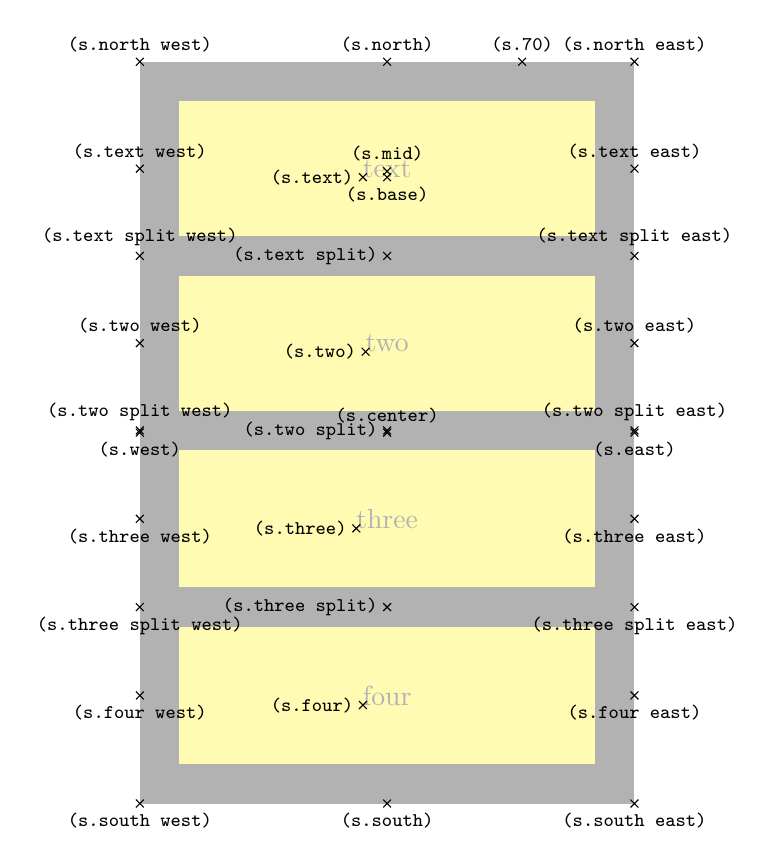
\begin{tikzpicture}
  \node[name = s, shape = rectangle split, rectangle split parts = 4, shape example,
    inner ysep = 0.75cm]{\nodepart{text}text\nodepart{two}two \nodepart{three}three\nodepart{four}four};

  \foreach \anchor/\placement in {
    text/left, text east/above, text west/above,
    two/left, two east/above, two west/above,
    three/left, three east/below, three west/below,
    four/left, four east/below, four west/below,
    text split/left, text split east/above, text split west/above,
    two split/left, two split east/above, two split west/above,
    three split/left, three split east/below, three split west/below,
    north/above, south/below, east/below, west/below,
    north west/above, north east/above, south west/below, south east/below,
    center/above, 70/above, mid/above, base/below}
    \draw[shift=(s.\anchor)] plot[mark=x] coordinates{(0,0)} node[\placement] {\scriptsize\texttt{(s.\anchor)}};
\end{tikzpicture}
\end{document}